%
% File acl2013.tex
%
% Contact  navigli@di.uniroma1.it
%%
%% Based on the style files for ACL-2012, which were, in turn,
%% based on the style files for ACL-2011, which were, in turn, 
%% based on the style files for ACL-2010, which were, in turn, 
%% based on the style files for ACL-IJCNLP-2009, which were, in turn,
%% based on the style files for EACL-2009 and IJCNLP-2008...

%% Based on the style files for EACL 2006 by 
%%e.agirre@ehu.es or Sergi.Balari@uab.es
%% and that of ACL 08 by Joakim Nivre and Noah Smith

\documentclass[11pt]{article}
\usepackage{acl2013}
\usepackage{times}
\usepackage{url}
\usepackage{latexsym}

\usepackage{graphicx}
%\setlength\titlebox{6.5cm}    % You can expand the title box if you
% really have to
%
\usepackage{hyperref}
\hypersetup{
    hidelinks=true,
    unicode=true,   % Enable the 21st century
    pdfborder={0,0,0,[]},
    pdfauthor={Stephen Wattam},
    linkbordercolor={0 0 0},
    citebordercolor={0 0 0},
    urlbordercolor={0 0 0},
    urlcolor=black,
    filecolor=black,
    citecolor=black,
    linkcolor=black,
    colorlinks=true,
    bookmarks=true
}


\newcommand{\toolname}{LWAC}
\newcommand{\superscript}[1]{{\small \ensuremath{^{\textrm{#1}}}}}
\newcommand{\subscript}[1]{{\small \ensuremath{_{\textrm{#1}}}}}
\newcommand{\citefn}[1]{\footnote{#1}}

\title{\toolname: Longitudinal Web-as-Corpus Sampling}

\author{Stephen Wattam\superscript{1}\\\And
  Paul Rayson\superscript{1}\\\And
  Damon Berridge\superscript{2}\\\AND
  Lancaster University\\
  School of Computing and Communications\superscript{1}, Mathematics and Statistics\superscript{2}\\
  {\tt f.lastname@lancs.ac.uk}\\
}


\date{}

\begin{document}
\maketitle

\section{Sampling}

Many sampling efforts for linguistic data on the web are heavily focused on producing results comparable to conventional corpora.  These typically take two forms: those based on URI lists (e.g. from search results, as in %~\cite{sharoff2006creating}
BE06~\cite{baker2009be06}, BootCat~\cite{baroni2004bootcat}), and those formed through crawling (e.g. enTenTen\citefn{\texttt{http://trac.sketchengine.co.uk/wiki/\\Corpora/enTenTen}}, %~\cite{}, %FIXME
UKWaC~\cite{ferraresi2008introducing}).

Though initial efforts in web-as-corpus (WaC) first focused on the former method %, in part due to concerns over the balance of samples returned, 
many projects are now focused on constructing supercorpora, which may themselves be searched with greater precision than the `raw' web, in line with Kilgarriff's vision of linguistic search engines~\cite{kilgarriff2003linguistic}.  This has led to the proliferation of crawlers such as those used in~\cite{schafer8building} and WebCorp\citefn{\texttt{http://www.webcorp.org.uk/live/
}}.%~\cite{renouf2003webcorp}.

% diachronic work with webcorp.
% \cite{kehoe2006diachronic}
% \cite{kehoe2009weaving}

This approach, with its base in a continually-growing supercorpus, parallels the strategy of a monitor corpus%~\cite{sinclair1982monitor}
, and is applicable to linguistic inquiry concerned with diachronic properties%~\cite{kehoe2006diachronic}
.
%Even for informal searches, tools for date-based lookup are increasingly (e.g. Google).


Repeated sampling by crawling, whilst balanced linguistically, omits subtler technical aspects that govern consumption of data online, most notably the user's impression of its location, as defined by the URI.  Low publishing costs online, paired with increasing corporate oversight and reputation management, (both personal %~\cite{ICT4DBibliography1650} 
and professional%~\cite{Malaga2000repman})
), have lead to a situation where this content is being revised frequently, often without users even noticing.

This URI-oriented change has been studied from a technical perspective by those interested in managing network infrastructure, compiling digital libraries%~\cite{tyler2003librarians}
, and optimising the maintenance of search engine databases%~\cite{koehler2004longitudinal}
.  The needs of these parties are quite aside from those of corpus researchers, however, since they focus around a best-effort database of information, rather than a dependable longitudinal sample with known margins for error.
% 
% \begin{itemize}
%     \item \textsl{Incremental sampling}---Search engine databases and digital archives are persistent, and may be incrementally updated in a continuous manner whilst still being useful;
%     \item \textsl{Lack of comparability}---A cross-sectional sample of search databses yields documents sampled at various times, with a possible age variation as modelled by the specific type of web page.  This is evidenced well by the relative likelihood of receiving a broken link when searching for current events \textsl{vs.} older scientific articles.
%     \item \textsl{Information-seeking behaviour}---Search engine literature indicates [CITE] that information, when lost from one location, is often available at many others.  This same process is unlikely to be followed, however, if a resource has simply changed, or if a user relies on a small set of web pages as an information resource (such as news sources).
%     \item \textsl{Deliberate `usefulness bias'}---Sources deemed to be pertinent to a search engine's clientelle are sampled more frequently, and thoroughly.  This results in persistence-of-value surrounding high-profile domain names and companies, which dominate the zipfian distribution of web results.
% \end{itemize}
% 


We present here a tool, \toolname, for this form of longitudinal sampling, designed to maximise the comparability of documents downloaded in each sample in terms of their URI rather than content.  To accomplish this, we use a batch-mode sampling strategy, as illustrated in Figure~\ref{fig:sampling}, to get full coverage over a list of URIs, at the expense of sampling new content.

\begin{figure}[h]
\centering
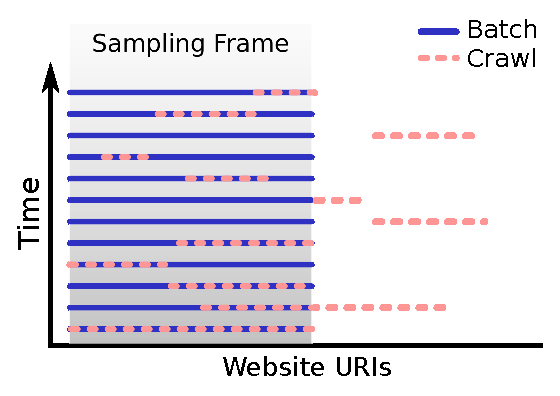
\includegraphics[width=0.4\textwidth]{images/samples.eps}
\caption{URI coverage for batch and crawl.}
\label{fig:sampling}
\end{figure}

\section{Applications}
Our strategy allows us to investigate how language may change in relation to technical and social events in a way that mimics the experience of the end user, and offers a useful perspective on many epistemic problems of WaC methods, to determine:

\begin{itemize}
    \item The portions of web pages that typically change as main content regions;
        \vspace{-6pt}
    \item The impact of social feedback and user generated content on page content;
        \vspace{-6pt}
    \item How censorship, redaction and revision affect website contents;
        \vspace{-6pt}
    \item Website resource persistence and its relation to linguistic content (link rot/document attrition);
        \vspace{-6pt}
    \item How institutions' publishing policies affect reporting of current events.
\end{itemize}

In order to maximise its coverage of these topics, \toolname~is designed to construct longitudinal samples from arbitrary URI lists, using commodity hardware, in a way that mimics the user's experience of a website.  


% The tool is designed to construct longitudinal samples from URI lists, using only commodity hardware.  It is designed with `full storage' in mind, that is, recording everything about each HTTP session in such a way that it may later be exported and accessed in a parsimonious manner.

\section{Architecture \& Performance}

\begin{figure}[h]
\centering
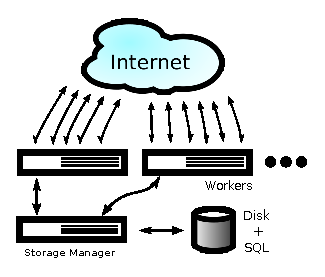
\includegraphics[width=0.4\textwidth]{images/arch.eps}
\caption{System Architecture}
\label{fig:arch}
\end{figure}

In order to form a useful longitudinal sample, each data point should be as time-invariate as possible.  As such, a highly parallel, distributed architecture was selected (Figure~\ref{fig:arch}).  This yields technical benefits in terms of throughput (especially where the internet connection is a bottleneck), flexibility, and the ability to differentiate between websites that are blocked for a given area of the internet and those that are offline proper.

Data storage in the system is split between metadata, stored in an SQLite database, and website sample data itself, which is stored as raw HTTP response data in a versioned structure, compressed using hard links\footnote{Linked in a similar manner to rsync's \texttt{-H} option.}.  The storage format is optimised for large samples, and is nested in order to avoid common filesystem limits.

The download process is managed by a central server, which co-ordinates storage and metadata access, and provides full atomicity.  This server distributes batch jobs, according to policies governing reliability and throughput, to worker clients, which compete for the opportunity to download web pages.

Workers imitate the behaviour of end users' browsers as much as possible, so as to avoid search engine optimisation and user-agent detection tactics: they retain cookies and present typical request headers.

% \section{Performance}
In order to obtain the most simultaneous samples, the system was designed to maximise the parallel number of connections on each client.  This is limited by the underlying OS, which in our tests showed a practical maximum of 120 simultaneous downloads\footnote{Using the Linux 2.8 kernel}.

In practice, throughput is limited by several factors, among them the available bandwidth, number of worker clients, speed of DNS lookups, and the proportion of links which are destined to time out during connection.  With favourable network conditions, each worker is capable of downloading a sample the size of the BE06 corpus in under a second.
% In testing, each worker proved capable of downloading at a sustained 8-12MBps, depending on job size and remote server properties.
% and use of two worker servers produces download rates of 0.2 to 0.3 million links an hour, with favourable remote server conditions.

% throughput is defined both by the external servers and this parallelism limit---reducing timeouts for failed DNS and HTTP connections leads to significant improvements later on in a sample where many hosts have fallen offline.  With low failure rates, the system is capable of downloading millions of pages in a 24-hour period.

% As with many downloaders, it is possible to exceed polite limits of server usage with an internet connection of even modest throughput.
% The original uses for the tool required sampling once or twice per server, meaning this was not a significant problem, however, those wishing to download websites will find themselves dealing with significant ethical concerns.

\section{Conclusion}
The \toolname~sampling tool, available online\footnote{\url{http://ucrel.lancs.ac.uk/LWAC/}}, offers an easy and rigorous way to compile longitudinal web corpora from arbitrary URI lists.  We believe it has particular utility to investigation of challenges that face WaC methods, as well as fine-grained sampling of language linked to current events and other fast-moving phenomena.

\vspace{-12pt}

\bibliographystyle{acl}
% you bib file should really go here 
\bibliography{downloadtools}

\end{document}
